\noindent
In order to start using the \curvgrid{} module we recommend to study the source code of the tutorials provided in \textit{curvilineargridhowto} folder. The tutorials use progressively more complicated concepts, so it is recommended to address them in the indexed order.


\subsection{Preliminaries - Creating Grid}
\label{usage-howto-tutorial-preliminaries}

All tutorials of \curvgrid{} reuse the simple auxiliary routine located in \textit{creategrid.hh}. This routine contains paths to all meshes currently used in tutorials, allowing the user to select the desired mesh by providing its index. It then proceeds to initialize the logging mechanisms
\begin{mybox}
\begin{lstlisting}
    Dune::LoggingMessage::init(mpihelper);
    Dune::LoggingTimer<Dune::LoggingMessage>::init(mpihelper);
\end{lstlisting}
\end{mybox}

\noindent
These singleton classes are essential for \curvgrid{}, as they support the parallel logging of the grid reading, construction and writing process, as well as later statistics on performance of individual routines. They can also be used by the user to write user logging output and time user functions, comparing them to the grid construction time. The next step is initializing the \textit{Curvilinear Grid Factory}

\begin{mybox}
\begin{lstlisting}
  Dune::CurvilinearGridFactory<GridType> factory(withGhostElements, withGmshElementIndex, mpihelper);
\end{lstlisting}
\end{mybox}

\noindent
where the boolean variable $withGhostElements$ determines whether the Ghost elements will be constructed and $withGmshElementIndex$ determines if the global element index from \gmsh{} is going to be reused by the grid (recommended). Otherwise, the index is automatically generated (see Tutorial 6 for discussion). After the above prerequisites, the curvilinear \gmsh{} reader is used to read the mesh file, partition it and write it to the provided grid factory.

\begin{mybox}
\begin{lstlisting}
  Dune::CurvilinearGmshReader< GridType >::read(factory, filename, mpihelper); 
\end{lstlisting}
\end{mybox}

\noindent
The \textit{Curvilinear Grid Factory} extends the interface of the standard dune grid factory, and therefore it will not work with other grids available in Dune. In order to achieve that, one must instead use the provided \textit{FactoryWrapper}. This wrapper class adheres to the standard grid factory interface, and disregards any process tag or curvilinear information provided by the curvilinear \gmsh{} reader. \\

\noindent
Finally, the grid is constructed, providing the user with the associated pointer. We note that the user must delete the grid pointer after use. %This is due to the fact that the factory used to create the grid ceases to exist before the grid itself.

\begin{mybox}
\begin{lstlisting}
  GridType *grid = factory.createGrid();
\end{lstlisting}
\end{mybox}

\subsection{Tutorial 1 - Getting started}
\label{usage-howto-tutorial-gettingstarted}

\noindent
This tutorial uses the above procedure to construct the \curvgrid{} by reading it from a \gmsh{} file. This and all other tutorials can be run both in serial and in parallel. First we define the grid

\begin{mybox}
\begin{lstlisting}
  typedef Dune::CurvilinearGrid<ctype, dim, isCached> GridType;
\end{lstlisting}
\end{mybox}

\noindent
where $dim=3$ is the dimension of the grid, $ctype=double$ is the underlying real type, and the $isCached$ is a boolean variable determining if the curvilinear geometry caching is used (recommended). Currently, only 3D tetrahedral grids are available. Then, the curvilinear grid is created by the $createGrid$ procedure described above. Finally, if we are interested in the time statistics for reading and construction of the grid, it can be obtained using the following command

\begin{mybox}
\begin{lstlisting}
  Dune::LoggingTimer<Dune::LoggingMessage>::reportParallel();
\end{lstlisting}
\end{mybox}



\subsection{Tutorial 2 - Traverse}
\label{usage-howto-tutorial-traverse}

This tutorial repeats the procedure from tutorial 1 to create the grid. It then iterates over the grid and extracts relevant information from the curvilinear entities. Currently, \curvgrid{} does not support refinement, so both leaf and level iterators will only iterate over the parent entities. As of \dune{} 2.4 revision the range-based for iterators introduced in \textit{c++11} standard are the preferred way to perform grid iteration. The below example iterator will iterate over all entities of the grid of a given codimension

\begin{mybox}
\begin{lstlisting}
  LeafGridView leafView = grid.leafGridView();
  for (auto&& elementThis : entities(leafView, Dune::Dim<dim - codim>())) {...}
\end{lstlisting}
\end{mybox}


Now, we would like to extract some relevant information from the iterator
\begin{mybox}
\begin{lstlisting}
  Dune::GeometryType gt = elementThis.type();
  LocalIndexType  localIndex
    = grid.leafIndexSet().index(elementThis);
  GlobalIndexType globalIndex
    = grid.template entityGlobalIndex<codim>(elementThis);
  PhysicalTagType physicalTag
    = grid.template entityPhysicalTag<codim>(elementThis);
  InterpolatoryOrderType interpOrder
    = grid.template entityInterpolationOrder<codim>(elementThis);
  BaseGeometry geom
    = grid.template entityBaseGeometry<codim>(elementThis);
  std::vector<GlobalCoordinate> interpVertices = geom.vertexSet()
\end{lstlisting}
\end{mybox}

\noindent
The $GeometryType$ and $LocalIndex$ are standard in \dune{}. $GlobalIndex$ provides a unique integer for each entity of a given codimension, over all processes. $PhysicalTag$ is the material tag associated with each entity, obtained from the mesh file. It can be used to relate to the material property of the entity, or to emphasize its belonging to a particular subdomain. In current \dunegrid{} standard this information can only be obtained by through the reader and requires auxiliary constructions. $InterpolatoryOrder$ denotes the integer polynomial interpolation order of the geometry of the entity. Currently, \curvgrid{} supports orders 1 to 5, the limiting factor being the curvilinear vertex indexing mapper in the reader. Finally, the $entityBaseGeometry$ gives the user direct access to the curvilinear geometry class of the entity, thus extending the interface provided by \textit{Dune::Grid::Geometry}. For example, it can be used to obtain the set of interpolatory vertices of the geometry, or an analytic polynomial matrix representing its Jacobian. \\






\subsection{Tutorial 3 - Visualization}
\label{usage-howto-tutorial-visualisation}

This tutorial demonstrates a simple way to output the curvilinear grid and associated vector fields (e.g. solutions of your PDE) to a PVTU file set using the \textit{CurvilinearVTKGridWriter} class. The writer is able to output arbitrary number of user-defined fields. The fields can be scalar or vector, and can be associated either with elements or with boundary faces. The sampled fields must overload the \textit{Dune::VTKScalarFunction} or \textit{Dune::VTKVectorFunction} standard provided by \curvgrid{}, and thus adhere to the following interface:

\begin{mybox}
\begin{lstlisting}
    // Writer initializes the functor once per each entity. This procedure can be used to pre-compute any quantities that do not change over the entity, accelerating the output
    virtual void init (const Entity & entity) {...}

    // Procedure that returns the field value as a function of local (!) coordinate
    virtual Range evaluate(const Domain & x) const  {...}

    // Procedure that returns the field name as it will appear in output file
    virtual std::string name() const  { return "localIndex2D"; }
\end{lstlisting}
\end{mybox}

\noindent
We provide 6 examples:
\begin{itemize}
  \item Element index scalar in 3D, written over all elements of the grid;
  \item Boundary segment index scalar in 2D, written over all boundary segments of the grid;
  \item Local sinusoidal vector in 3D, written over all elements of the grid;
  \item Local sinusoidal vector in 2D, written over all boundary segments of the grid;
  \item Global sinusoidal vector in 3D, written over all elements of the grid;
  \item Global sinusoidal vector in 2D, written over all boundary segments of the grid;
\end{itemize}

\noindent
These examples illustrate the important difference between local and global coordinates. Local coordinates are unique for each element, so one shall observe unique field behavior for each element. Global coordinates on the other hand are the same for all elements, thus providing a single continuous sinusoid across the entire mesh. The local fields are associated with the orientation of the element in space, which is arbitrary up to the permutation of element corners. Thus, to correctly display local fields, one must consider the orientation of the element. This can be achieved by considering the global coordinates and/or global indices of the corner vertices of the element, and of the intersection faces in between two elements. \\

\noindent
We start by constructing a curvilinear grid as previously demonstrated. We then proceed to initialize the writer, as well as fix its virtual refinement order to 15. We do this because we want to resolve the details of the sinusoid function to a very high precision, and because the mesh size is small. This operation is time-consuming, and, in general, the user should be aware of quadratic complexity of virtual refinement, and choose the refinement order that is necessary and sufficient. Should we choose to avoid specifying a fixed refinement order, the writer will calculate this order itself by considering the curvilinear order of the element. This works fine for most FEM applications, unless the basis order of the element is larger than its curvilinear order.

\begin{mybox}
\begin{lstlisting}    
  Dune::CurvilinearVTKGridWriter<GridType> writer(*grid);
    
  const int userDefinedVirtualRefinement = 15;
  writer.useFixedVirtualRefinement(userDefinedVirtualRefinement);
\end{lstlisting}
\end{mybox}

\noindent
We proceed to stack the pointers to the above field functors into 4 arrays, distinguished by vector/scalar and 2D/3D fields. We have decided to use dynamic polymorphism to implement this functionality. While this may be less efficient than other implementations, it allows writing fields produced by different functors by the very same compact routine.

\begin{mybox}
\begin{lstlisting}    
  std::vector<BaseVTKScalarFunction2D *> vtkFuncScalarSet2D_;
  std::vector<BaseVTKScalarFunction3D *> vtkFuncScalarSet3D_;
  std::vector<BaseVTKVectorFunction2D *> vtkFuncVectorSet2D_;
  std::vector<BaseVTKVectorFunction3D *> vtkFuncVectorSet3D_;

  vtkFuncScalarSet2D_.push_back(
    new VTKFunctionBoundarySegmentIndex<GridType>(*grid));
  vtkFuncScalarSet3D_.push_back(
    new VTKFunctionElementIndex<GridType>(*grid));

  vtkFuncVectorSet2D_.push_back(new VTKFunctionLocalSinusoidFace());
  vtkFuncVectorSet2D_.push_back(new VTKFunctionGlobalSinusoidFace());
  vtkFuncVectorSet3D_.push_back(new VTKFunctionLocalSinusoidElem());
  vtkFuncVectorSet3D_.push_back(new VTKFunctionGlobalSinusoidElem());

  writer.addFieldSet(vtkFuncScalarSet2D_);
  writer.addFieldSet(vtkFuncScalarSet3D_);
  writer.addFieldSet(vtkFuncVectorSet2D_);
  writer.addFieldSet(vtkFuncVectorSet3D_);
  writer.write("./", "tutorial-3-output"););
\end{lstlisting}
\end{mybox}
	
	
\begin{figure}[H]
	\begin{subfigure}[b]{0.45\textwidth} \hspace{4mm} 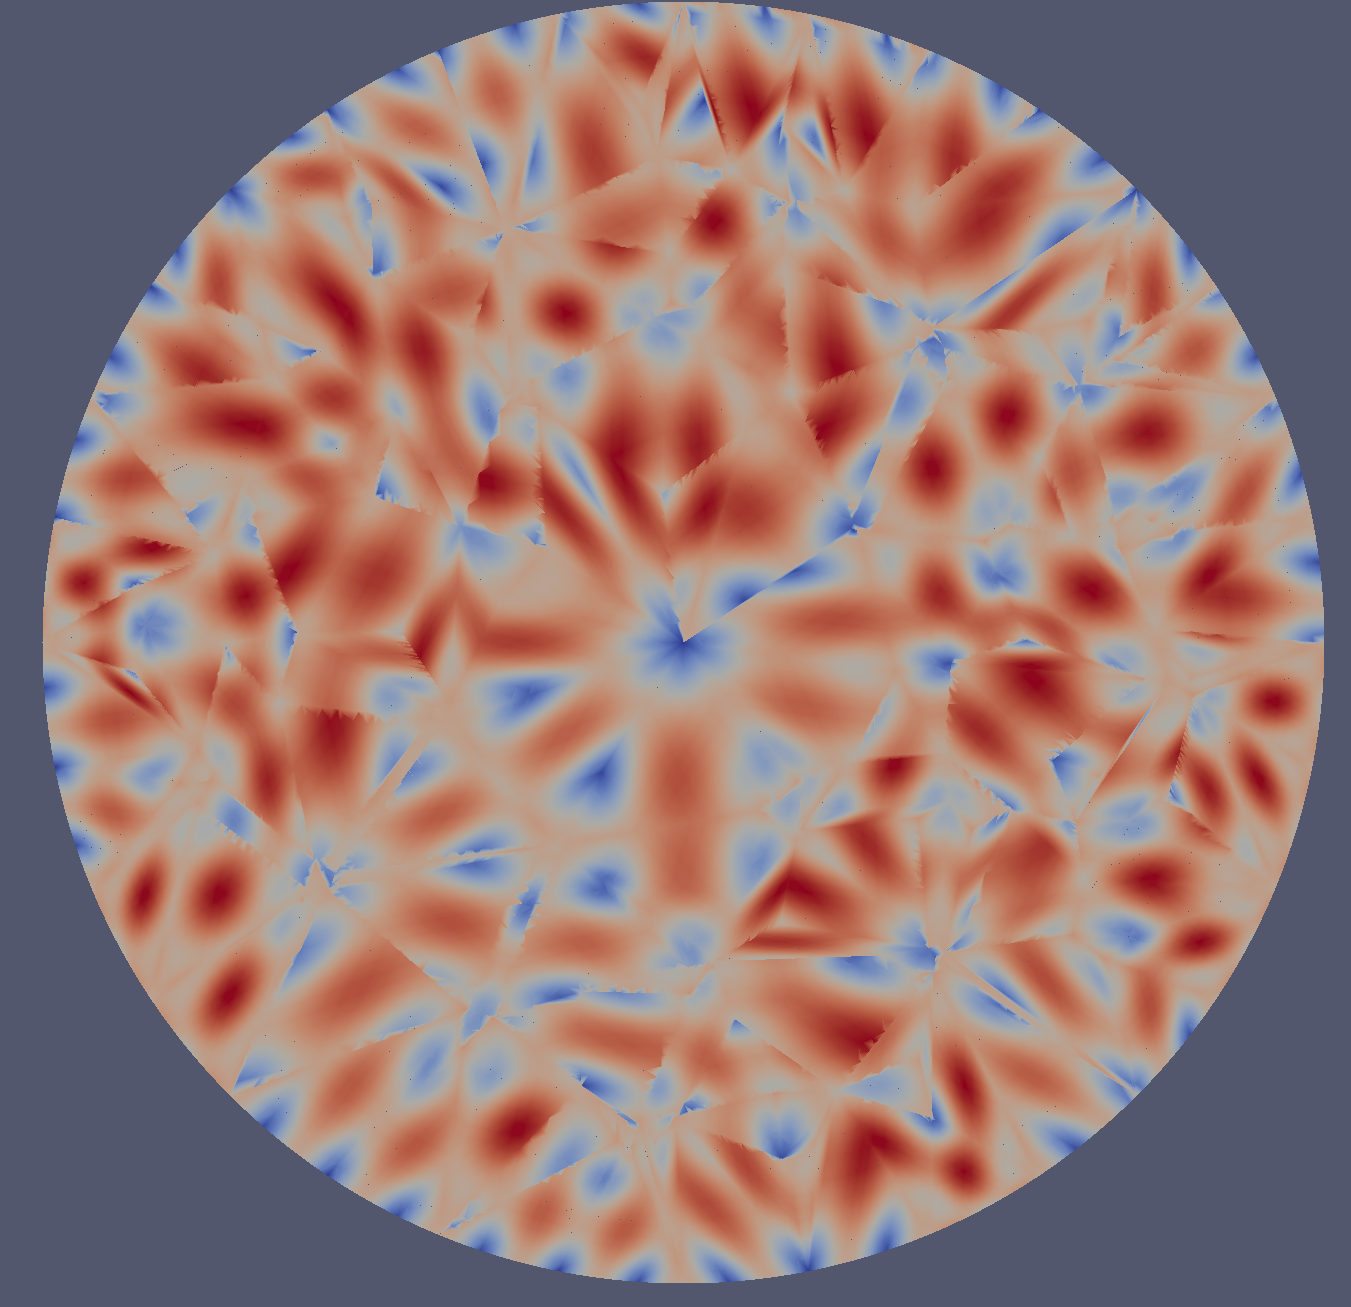
\includegraphics[scale=0.14]{images/tutorial3-vtk-localsinusoid} \end{subfigure}
	\begin{subfigure}[b]{0.45\textwidth} \hspace{4mm} 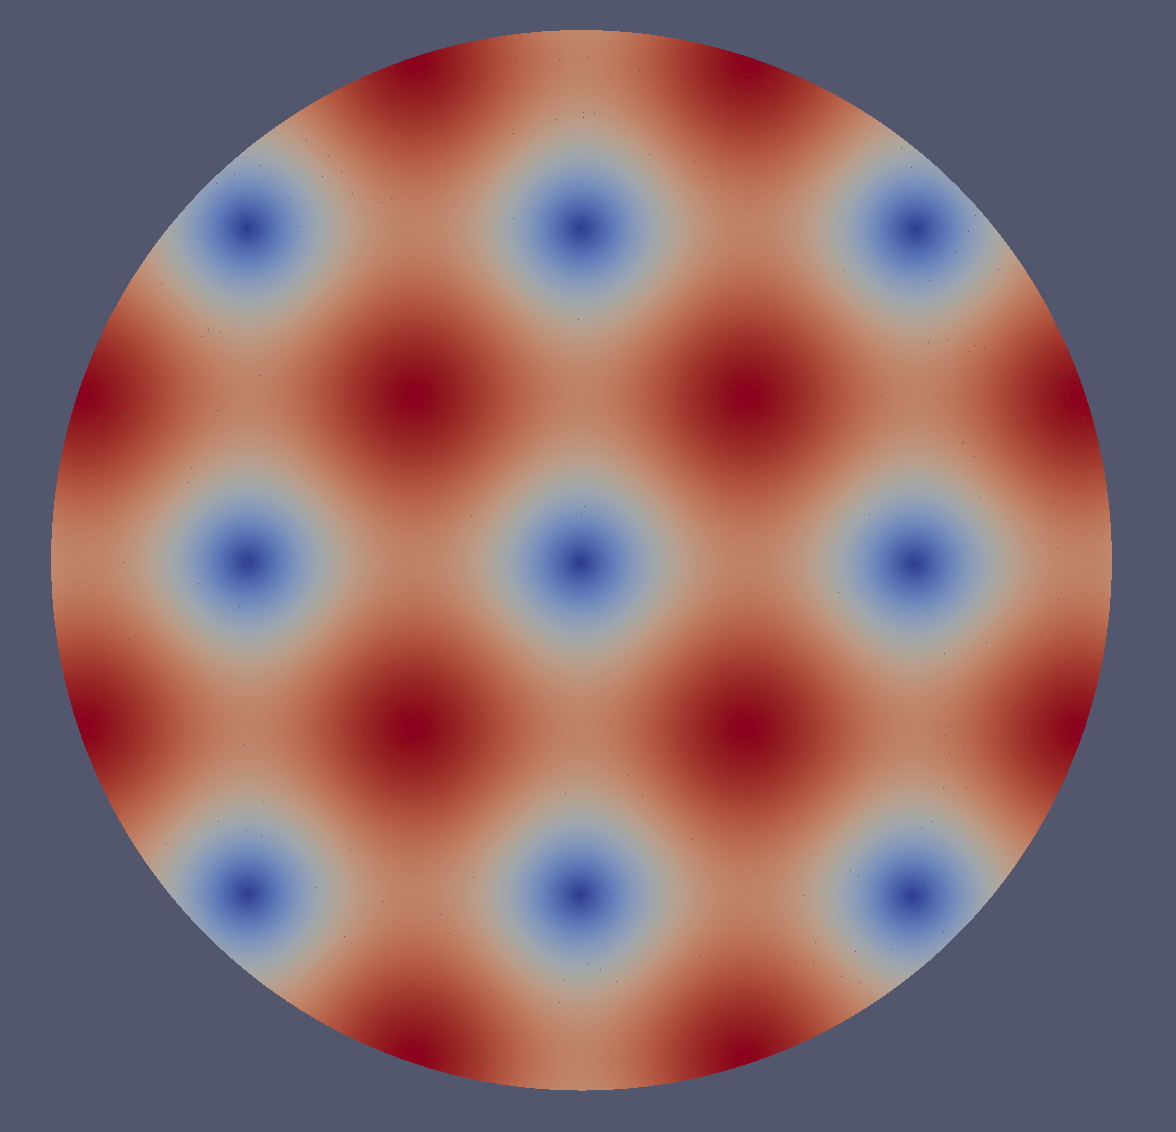
\includegraphics[scale=0.16]{images/tutorial3-vtk-globalsinusoid} \end{subfigure}
	\caption{ Visualization of tutorial 3. A sinusoid as function of local and global coordinates. This example emphasizes that there is no a priori orientation of the local coordinates. It is the task of the user to ensure that the local field is correctly oriented by considering the global indices of intersecting entities.}
	\label{fig:tutorial3:sinusoid}
\end{figure}


\subsection{Tutorial 4 - Quadrature Integration Tutorials}
\label{usage-howto-tutorial-integration-quadrature}

The following two tutorials demonstrate the capability of \curvgrid{} to address mathematical and physical problems requiring integration of certain quantities over the grid domain. \\


\noindent
\textbf{Scalar Surface Integral - \textit{Gauss} Law} \\
%
\noindent
In this example we verify \textit{Gauss} law numerically by computing the surface integral of the electric field produced by a unit point charge across the domain boundary of the mesh enclosing that charge. The tutorial will demonstrate that changing the curvature of the domain boundary or the position of the charge inside the domain does not affect the result that is $4 \pi$. More precisely, we compute the integral
\[\int_{\delta \Omega} \vec{E}(\vec{x}) \cdot d\vec{S} = \int_{\delta \Omega} \vec{E}(\vec{x}(\vec{u})) \cdot \vec{n}(\vec{u}) I(\vec{u}) d^2 u \]
\noindent
where $\vec{x}$ is the global coordinate, $\vec{u}$ is the coordinate local to the surface finite element,
\[\vec{E}(\vec{x}) = \frac{\vec{x} - \vec{x}_0}{|\vec{x} - \vec{x}_0|^{-3}}\]
is the electric field of a unit charge located at $\vec{x}_0$, $\vec{n}(\vec{u})$ is the surface outer normal in global coordinates as a function of local coordinates and
\[I(\vec{u}) = \sqrt{\det [ J^T(\vec{u}) J(\vec{u}) ]}\]
is the generalized integration element due to conversion of the integral from global to local coordinates (see \cref{appendix:integrationelements:proof}). \\

\noindent
In order to use the \curvgeom{} integration capabilities, the user must provide the integrand in the form of a functor class. The functor need not be overloaded, but must implement the $()$ operator

\begin{mybox}
\begin{lstlisting}
  ResultType operator()(const LocalCoordinate & x) const {...}
\end{lstlisting}
\end{mybox}

\noindent
as a function of the coordinate local to the entity it is evaluated over, in this case, a 2D coordinate local to a face. The code then iterates over all domain boundaries of the grid, calculating integrals of the functor over each boundary segment and adding up the results. In order to integrate a functor, the \textit{QuadratureIntegrator} class needs to be provided with the entity geometry, the functor to be integrated, the relative and absolute tolerances to be used for integration, as well as the norm type to be used for the case of multidimensional integration. 
\begin{mybox}
\begin{lstlisting}
  typedef Dune::QuadratureIntegrator<ct, DIM2D>  Integrator2DScalar;
  typedef typename Integrator2DScalar::template Traits<Integrand2D>::StatInfo  StatInfo;	
  StatInfo thisIntegralG = Integrator2DScalar::template integrateRecursive<FaceGeometry, Integrand2D, NORM_TYPE>(geometry, gaussf, RELATIVE_TOLERANCE, ACCURACY_GOAL);
\end{lstlisting}
\end{mybox}

\noindent
\textit{StatInfo} is the return data type of the \textit{QuadratureIntegrator}, which is a pair of the integral result and the quadrature order at which the desired relative accuracy was achieved. Note that the absolute accuracy \textit{ACCURACY\_GOAL} is used to determine if the integral is close enough to 0, as relative accuracy can not be used for this purpose due to division by 0. \\



\noindent
\textbf{Surface Vector Integral - Normal Integral} \\
%
\noindent
This test demonstrates the capability of \textit{QuadratureIntegrator} to integrate vector quantities. It tests the well-known identity, stating that the integral over the unit outer normal over a closed bounded domain is 0.

\begin{equation}
	\oiint_{\partial \Omega} n_x dS = \oiint_{\partial \Omega} \vec{e}_x \cdot \vec{n} dS = \iiint_{\Omega} \nabla \cdot \vec{e}_x dV = 0
\end{equation}

\noindent
The implementation of this test is almost identical to the \textit{Gauss} integral test above. The only difference is that \textit{Dune::FieldVector} is used as a functor output, and internally, instead of taking the dot product between the outer normal and the electric field, the normal itself is returned


%\subsection{Tutorial 4 - Recursive Numerical Integration}
%\label{usage-howto-tutorial-integration-recursive}


\subsection{Tutorial 5 - Communication via the DataHandle Interface}
\label{usage-howto-tutorial-communication}

This tutorial, consisting of two parts, serves as a simple use-case of interprocessor communication through grid entities, which is achieved via the \textit{DataHandle} interface. \\

\noindent
In the first tutorial we explicitly select all entities of the grid that are supposed to communicate for each available communication protocol, and communicate a dummy constant. The goal is to confirm that all the expected entities were communicated over, and all others were not. In the second tutorial, the global index of each entity is sent according to the specified communication protocol, and compared to the global index on the receiving side. It is demonstrated that these indices match for each communicating pair, and an exception is thrown should this not be the case. \\

% \noindent
% Briefly, the procedure communicateConstant iterates over all process process boundary intersections, and marks its neighbour entities, if they will be sending or receiving within the provided interface. Then the custom DataHandleConst is used to perform the communication. This data handle communicates one and the same constant to all entities it is requested. The important thing is that whenever gather or scatter methods are called, it checks if the requested entity was marked for sending or receiving, and throws an error if it is not. Finally, the main procedure checks that the total number of entities that have received the constant is equal to the number of entities marked for receiving.

\noindent
\curvgrid{} implements the \textit{DataHandle} communicators in accordance to the standard \dune{} interface, and its functionality does not exceed that envisioned by the standard interface. Since these tutorials are rather involved, and the standard mechanism is well-documented within the standard \dune{} reference, the detailed explanation of these two tutorials is beyond the scope of this paper. For further information, the user is referred to the \textit{Dune Grid Howto} documentation, found in \url{www.dune-project.org}



\subsection{Tutorial 6 - Parallel Data Output}
\label{usage-howto-tutorial-paralleldataoutput}

This tutorial demonstrates the use of a small utility \textit{ParallelDataWriter} designed for sorted parallel output of vectors. It explores the benefits of using the global element index provided by the mesh, for debugging of parallel numerical codes. The tutorial demonstrate that a quantity sampled over all elements of the grid and sorted by the element global index is independent of the number of processes used. Thus, the user can directly compare the output file, generated by runs with varying process count. \\

\noindent
\textit{Important Note: This tutorial only works if the mesh-provided global element index is re-used by the curvilinear \gmsh{} reader (default). If this is not the case, the automatically generated global index will depend on the number of processes and destroy the above symmetry.}

\noindent
This tutorial samples the volume of the elements. However, the interface of the \textit{ParallelDataWriter} extends to writing vectors of data for each element as well. One must first define the class

\begin{mybox}
\begin{lstlisting}
  <class Grid, class IndexType, class DataType>
  class ParallelDataWriter
\end{lstlisting}
\end{mybox}

\noindent
where \textit{IndexType} and \textit{DataType} are the data types of index and data arrays respectively. They can be any of the Plain Old Datatype (POD) classes, as long as their size is fixed over all processes for the communication purposes. One would then proceed to call the writer routine

\begin{mybox}
\begin{lstlisting}
  static void writeParallelData2File(std::string filename, std::vector<IndexType> & interiorElementGlobalIndex, std::vector<int> & interiorElementNDof, std::vector<DataType> & data, const Grid & grid)
\end{lstlisting}
\end{mybox}

\noindent
where \textit{interiorElementNDof} denotes the number of data entries per global index, and \textit{data} stores all data entries for all global indices in a contiguous 1D vector. \\


\subsection{Tutorial 7 - Global Boundary Communicator}
\label{usage-howto-tutorial-globalboundarycommunicator}

\noindent
This tutorial demonstrates the capabilities of \curvgrid{} to handle dense boundary communication problems, such as the Boundary Integral (BI) method. In the BI method, the global matrix or part of it correspond to pairwise coupling of every two faces on a given closed surface, providing a fully populated, i.e. dense, matrix. Each processor needs to obtain complete information of all faces on a given surface, collected over all processes.

\begin{mybox}
\begin{lstlisting}
  typedef Dune::CurvGrid::GlobalBoundaryContainer<GridType> BoundaryContainer;
  BoundaryContainer container(*grid, isDomainBoundary, volumeTag, surfaceTag);
\end{lstlisting}
\end{mybox}

\noindent
In case \textit{isDomainBoundary} is set to true, the \textit{BoundaryContainer} does not require the last two parameters. Otherwise, one must specify the surface tag of the interior surface, as well as the volume tag of elements either on the interior or the exterior of the surface, all one or the other. The unit outer normal for each face of the surface is determined as the unit outer normal of the associated element. Thus, if one provides the volume tag of the elements on the outside of the interior surface, one will always receive the inner unit normal at a later stage, and will have to multiply all of them by -1 in order to obtain the unit outer normal. The \textit{BoundaryContainer} does not contain the surfaces already located on this process, in order to save space.  \\

\noindent
In order to iterate over the \textit{BoundaryContainer}, we implement the accompanying \textit{BoundaryIterator}

\begin{mybox}
\begin{lstlisting}
  BoundaryIterator iter(container);
  while (!container.end()) {...}
\end{lstlisting}
\end{mybox}

\noindent
The boundary iterator re-implements most of the functionality of the standard Dune iterator, such as \textit{geometry()}, \textit{unitOuterNormal()}, \textit{indexInInside()}, \textit{geometryInInside()}, as well as some additional functionality compactified into the same iterator to save on communication complexity, such as 

\begin{mybox}
\begin{lstlisting}
  template <int codim>
  UInt globalIndex(UInt subIndexInFace) const {...}

  template <int codim>
  UInt globalIndexInParent(UInt subIndexInElem) const 

  UInt order() const { }

  BaseGeometryEdge geometryEdge(UInt subIndex) const {..}
\end{lstlisting}
\end{mybox}

\noindent
The tutorial performs several tests of the communicated boundary, such as the normal integral from Tutorial 4, calculation of total number of edges, as well as the complementarity of the global index of boundary surfaces located on this process, and on the \textit{BoundaryContainer}. \\




\subsection{Tutorial 8 - Interior Boundary}
\label{usage-howto-tutorial-interiorboundary}

The tutorial extends the \textit{Gaussian} integral tutorial to interior boundaries, performing integrals for a set of charges inside and outside of the boundary. This is a simple test to verify if the interior boundary of the mesh forms a closed surface.



\subsection{Tutorial 9 - Periodic Boundary}
\label{usage-howto-tutorial-periodic}

This tutorial is meant to convince the user that the periodic boundaries really correspond to each other, including correct rotation. Consider that a solution for some PDE, which is periodic along $x$ and $y$, is $F(\vec{x}) = \sin(k \vec{e}_z \cdot \vec{x})$, where $k$ is the wavenumber and $\vec{e}_z$ is the $z$ unit vector. This solution is expected to match across $x$ and $y$ periodic planes. In order to quantify the error of such mismatch, the user might want to compute the following integral for each triangle $\Delta$

\[
  \epsilon_\Delta = \iint \biggl | F(\vec{g}^{\Delta}_{in}(\vec{u})) - F(\vec{g}^{\Delta}_{out}(\vec{u})) \biggr | d^2u
\]

\noindent
where $u$ is a reference triangle local coordinate, $\vec{g}^{\Delta}_{in}$ is the global coordinate within the triangle $\Delta$, and $\vec{g}^{\Delta}_{out}$ is the global coordinate within the periodic neighbour coordinate. It is very important that the global coordinates $\vec{g}^{\Delta}_{in}$ and $\vec{g}^{\Delta}_{out}$ are periodically-corresponding, otherwise the integral will not make any sense, regardless of whether the solution is right or wrong. As described in \cref{impl-grid-constructor-periodic}, the global coordinates are obtained via local geometry mappings \textit{geometryInInside} and \textit{geometryInOutside}. Please consider the evaluation routine of the $\sin$ error functor, implemented in this tutorial

\begin{mybox}
\begin{lstlisting}
const Intersection & I_;

ResultType operator()(const LocalCoordinate & xLocal) const
{
    LocalCoordinateParent xLocalInner = I_.geometryInInside().global(xLocal);
    LocalCoordinateParent xLocalOuter = I_.geometryInOutside().global(xLocal);

    GlobalCoordinate xGlobalInner = I_.inside().geometry().global(xLocalInner);
    GlobalCoordinate xGlobalOuter = I_.outside().geometry().global(xLocalOuter);

    ct fieldInner = sineField(xGlobalInner);
    ct fieldOuter = sineField(xGlobalOuter);

    return ResultType{fabs(fieldInner - fieldOuter)};
}
\end{lstlisting}
\end{mybox}

\noindent
In this tutorial we construct three $\sin$ functions, one for each coordinate axis, and integrate the solution error over all faces the other two dimensions. Since the solution given in the tutorial is exact, one will expect the error to be negligible. We observe the error of the order $10^{-15}$. Note that as the wavenumber $k$ increases, the $\sin$ function varies faster, and the integrator finds it more difficult to converge. For $k=10$ the integrator will complain that the maximal available integration order (61) is exceeded before reaching the desired relative accuracy. Higher order solution is directly correlated with higher order requirements for the integration order.




%%\subsection{Tutorial 5 - Polynomial Manipulation and Integration}
%%\label{usage-howto-tutorial-polynomial}
%%
%%
%%\subsection{Tutorial 7 - Point Location - OCTree}
%%\label{usage-howto-tutorial-octree}










